\documentclass[final,hyperref={pdfpagelabels=false},xcolor=table]{beamer}
\mode<presentation>{
	\usetheme{ucb}
}
\usepackage[size=custom,width=101.6,height=76.2,scale=1.5]{beamerposter}
\usepackage{multicol}
\usepackage{graphicx}
\usepackage{textcomp}
%\usepackage{booktabs}
%\usepackage{multirow}
%\usepackage{listings}
%\usepackage{siunitx}
\usepackage{blindtext}
\usepackage{pbox}

\graphicspath{{../figures/}}

\definecolor{ucb-pacific}{HTML}{5B6770}

\newcommand{\uT}{{\textmu}T}
\setlength{\leftmargini}{4em}

\title{Nephele: A Simple Solution for Data Replication}
\author{Joao Carreira, Howard Mao, and Nathan Pemberton}
\advisor{Randy Katz}
\institute[UC Berkeley]{\textsc{University of California, Berkeley}}

\begin{document}
\begin{frame}
\vspace{-1.5em}
\begin{columns}[t]
	\begin{column}{0.3\linewidth}
            \begin{block}{Motivation}
    As the number of nodes in distributed systems increases, failures become
    the rule, not the exception. Because of this, it is important to be able to
    recover from crashes quickly and with minimal impact on performance and
    complexity. Checkpointing and manual serialization/deserialization are both
    slow and complicated.
\end{block}

            \vspace{1ex}
            \begin{block}{Architecture}
    \centering
    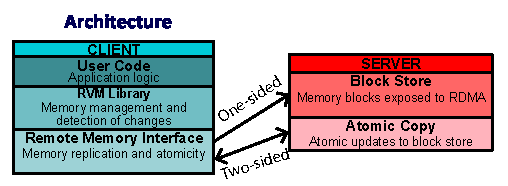
\includegraphics[width=0.9\textwidth]{lasagna.pdf}
\end{block}

            \vspace{1ex}
            \begin{block}{RVM API}
    RVM allows the user to allocate recoverable regions of memory and
    atomically replicate changes to that memory to a remote node’s DRAM. The
    user simply identifies recovery points in their code through a
    transactional API.

    \begin{itemize}
        \item \verb|rvm_cfg_create()| - Initialize the system and recover
            memory if needed.
        \item \verb|rvm_alloc()| - Allocate a region of recoverable memory.
        \item \verb|rvm_free()| - Free a region of recoverable memory.
        \item \verb|rvm_txn_start()| - Mark the beginning of a transaction.
        \item \verb|rvm_txn_commit()| - Atomically commit any changes made
            to recoverable memory since the last call to \verb|rvm_txn_start()|.
    \end{itemize}
\end{block}

            \vspace{1ex}
            \begin{block}{Backends}
    Underneath the RVM layer is a remote memory backend, which handles
    communication with the remote node. The rmem layer implements basic
    functions like \texttt{malloc()}, \texttt{free()}, \texttt{put()},
    \texttt{get()}, and \texttt{commit()}. So far we have implemented two
    different backends. One uses a custom protocol based on Infiniband RDMA.
    The other uses RAMCloud, an Infiniband-based key-value store.
\end{block}

	\end{column}

	\begin{column}{0.3\linewidth}
            \begin{block}{Micro-Benchmarks}
    \begin{itemize}
        \item In the micro-benchmarks, we measure how long it takes to commit
            changes to a set of pages and how long it takes to recover a set
            of pages after a crash.
        \item Took measurements for both backends and compared with BLCR.
        \item Commit latency increases linearly with number of pages.
        \item Recovery latency also increases, but not as neatly.
    \end{itemize}

    \vspace{1em}

    \centering
    \includegraphics[width=\textwidth]{commit-results.pdf}

    \includegraphics[width=\textwidth]{recovery-results.pdf}
\end{block}

	\end{column}

	\begin{column}{0.3\linewidth}
            \begin{block}{Macro-Benchmarks}
    \begin{itemize}
        \item \textbf{DGEMV} - Multiply a matrix by a vector and repeat using
            the result. We run using a 100,000 x 100 matrix over 1000
            iterations.  We measure how the total runtime is affected by
            failure rate (the number iterations between restarts) and commit
            rate (number of iterations between commits) and compare the
            results to simply saving the data to a file.
        \item \textbf{Gene Assembly} - Assemble gene sequences from a set of
            k-mers (fixed size gene sequences). We measure how the total
            runtime is affected by commit rate and compare the results to
            process state checkpointing using BLCR.
    \end{itemize}

    \centering

    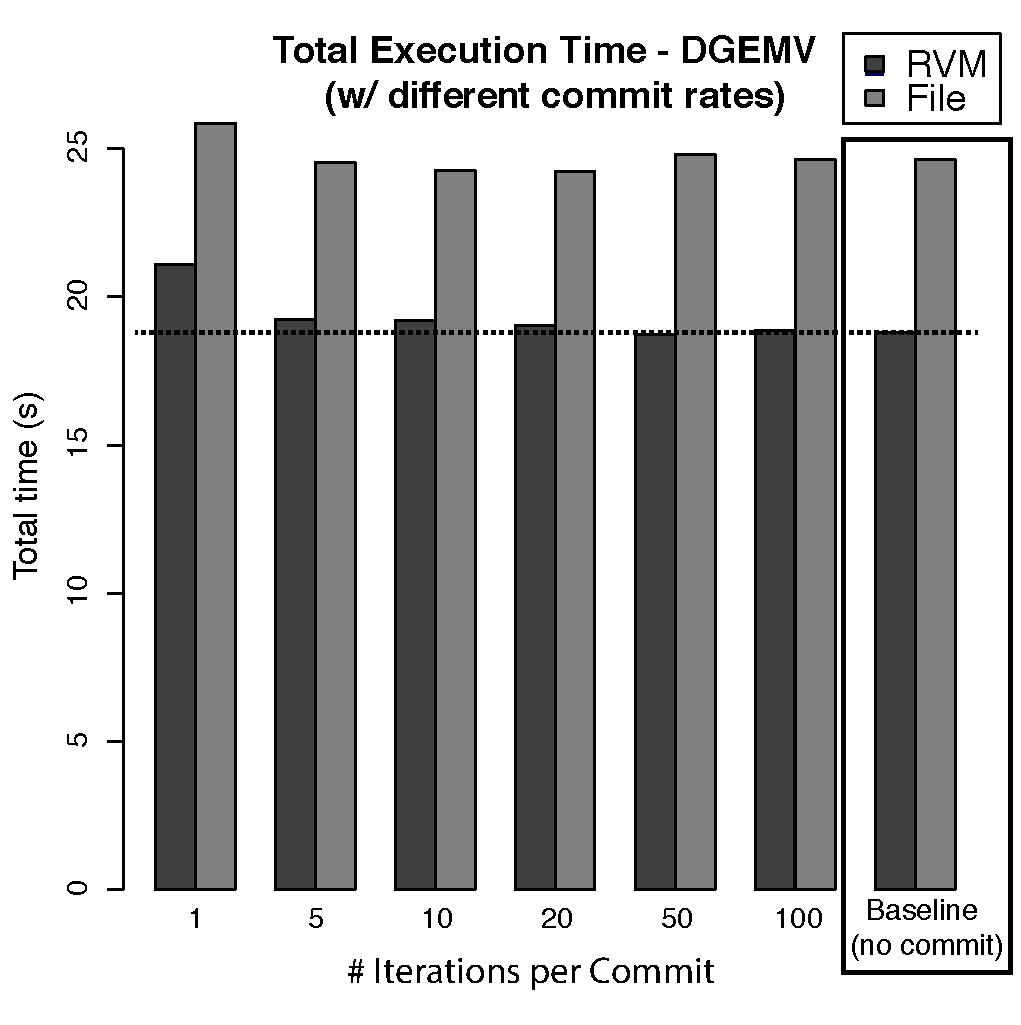
\includegraphics[width=0.45\textwidth]{dgemv_total_time_commit.pdf}
    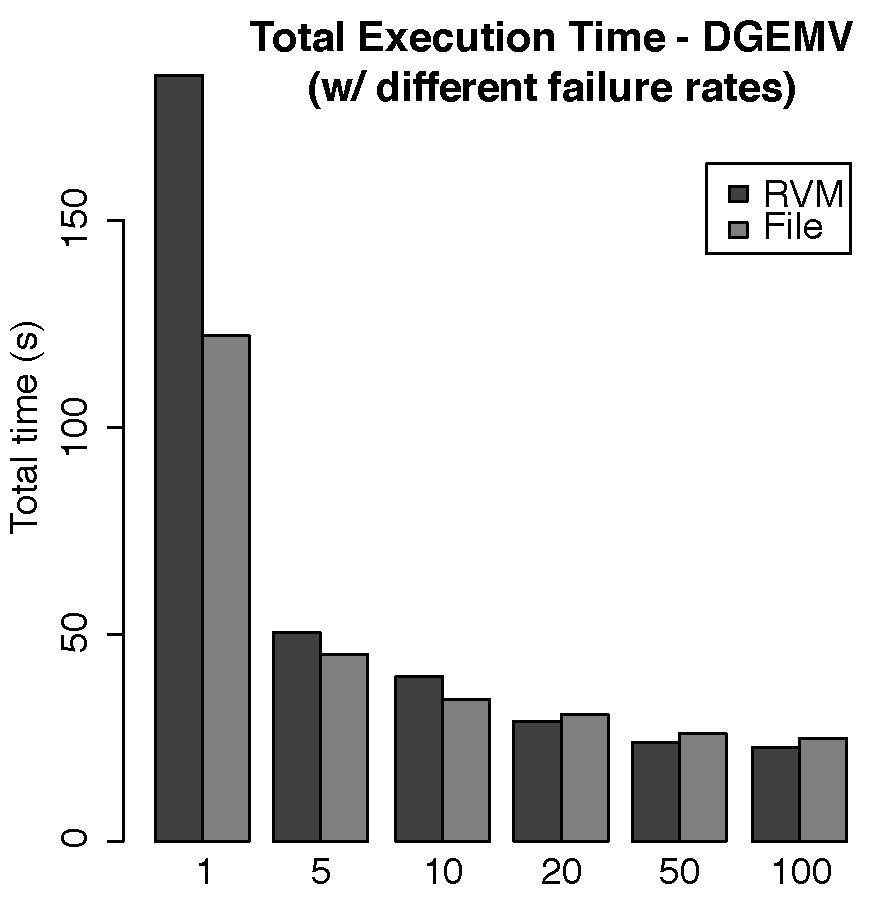
\includegraphics[width=0.45\textwidth]{dgemv_total_time_fail.pdf}

    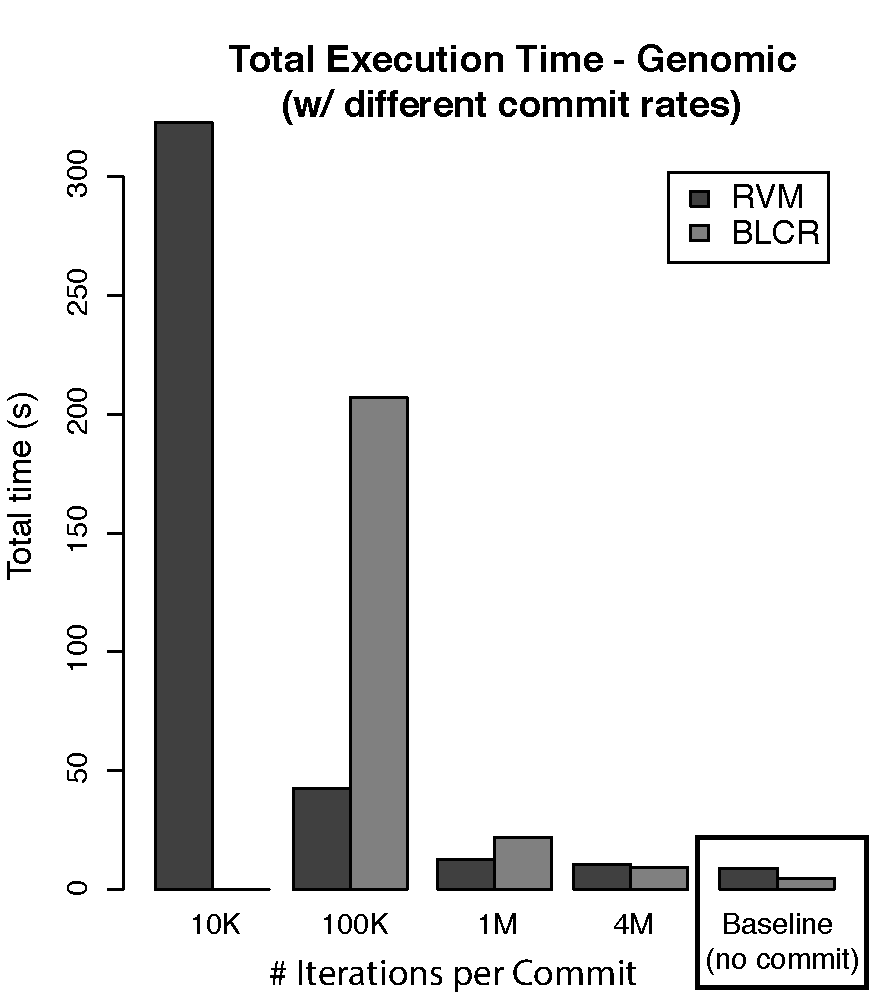
\includegraphics[width=0.45\textwidth]{genome_total_time_commit.pdf}
\end{block}

            \vspace{1ex}
            \begin{block}{Conclusion}
    Our library is able to provide checkpoints with microsecond latencies over
    complex in-memory data structures. In the case of DGEMV, natural runtime
    variation completely masked the effect of frequent checkpointing. The
    changes required to accommodate rvm were minimal, especially when compared
    to manual serialization. In the case of the genome benchmark, we were
    able to checkpoint a complicated data structure with lots of pointer with
    minimal effort. However, with such a large number of pages being changed,
    commit latency increased considerably. We still have a ways to go in
    improving performance.
\end{block}

	\end{column}
\end{columns}
\end{frame}
\end{document}
